
\documentclass[submit]{harvardml}


% You don't need to change these.
\course{CS181-S18}
\assignment{Assignment \#4}
\duedate{11:59pm March 30, 2018} % FDV: Update due date 

\usepackage[OT1]{fontenc}
\usepackage[colorlinks,citecolor=blue,urlcolor=blue]{hyperref}
\usepackage[pdftex]{graphicx}
\usepackage{subfig}
\usepackage{fullpage}
\usepackage{amsmath}
\usepackage{amssymb}
\usepackage{color}
\usepackage{todonotes}
\usepackage{listings}
\usepackage{common}
\usepackage{bm}
\usepackage{booktabs}
\usepackage{float}
\usepackage{graphicx}
\usepackage{float}
\usepackage{subfig}
\usepackage{cleveref}
\usepackage{adjustbox}


% http://www.tablesgenerator.com/#

\usepackage[mmddyyyy,hhmmss]{datetime}

\definecolor{verbgray}{gray}{0.9}
\definecolor{answergreen}{rgb}{0.09,0.42,0.31}

\newenvironment{answer}{%
    \color{answergreen}\bf}

\lstnewenvironment{csv}{%
  \lstset{backgroundcolor=\color{verbgray},
  frame=single,
  framerule=0pt,
  basicstyle=\ttfamily,
  columns=fullflexible}}{}


\newcommand{\bx}{\mathbf{x}} %%%% WARNING: may cause unexpected behavior
\newcommand{\by}{\mathbf{y}} %%%% WARNING: may cause unexpected behavior

%\newcommand{\bw}{\mathbf{w}} %%%% WARNING: may cause unexpected behavior
%\newcommand{\bS}{\mathbf{S}} %%%% WARNING: may cause unexpected behavior

%\newcommand{\mBI}{\mathbb{I}_{ik}} %%%% WARNING: may cause unexpected behavior
%%\newcommand{\bpi}{\mathbf{\pi}} %%%% Already built into latex 

%%\newcommand{\bmu}{\mathbf{\mu}} %%%% Already built into latex 
%\newcommand{\bvar}{\mathbf{\sigma}^2} %%%% WARNING: may cause unexpected behavior
\newcommand{\bSig}{\mathbf{\Sigma}} %%%% WARNING: may cause unexpected behavior
%\newcommand{\lsum}{\mathlarger{\sum}} %%%% WARNING: may cause unexpected behavior


\begin{document}
\begin{center}
{\Large Homework 4: Clustering and EM}\\
\end{center}


This homework assignment focuses on different unsupervised learning
methods from a theoretical and practical standpoint.  In Problem 1,
you will explore Hierarchical Clustering and experiment with how the
choice of distance metrics can alter the behavior of the algorithm. In
Problem 2, you will derive from scratch the full
expectation-maximization algorithm for fitting a Gaussian mixture
model. In Problem 3, you will implement K-Means clustering on a
dataset of handwritten images and analyze the latent structure learned
by this algorithm.

There is a mathematical component and a programming component to this
homework.  Please submit your PDF and Python files to Canvas, and push
all of your work to your GitHub repository. If a question requires you
to make any plots, please include those in the writeup.



\newpage
\section*{Hierarchical Clustering [7 pts]}

At each step of hierarchical clustering, the two most similar clusters
are merged together. This step is repeated until there is one single
group. We saw in class that hierarchical clustering will return a
different result based on the pointwise-distance and cluster-distance
that is is used. In this problem you will examine different choices of
pointwise distance (specified through choice of norm) and cluster
distance, and explore how these choices change how the HAC algorithm
runs on a toy data set.


\vspace{0.25cm}

\begin{problem}
~

 Consider the following four data points in $\reals^2$, belonging to three clusters: the
  black cluster consisting of $\boldx_1 = (0.1, 0.5) $ and $\boldx_2 = (0.35, 0.75))$,
  the red cluster consisting of $\boldx_3 = (0.28, 1.35)$, and the blue cluster
  consisting of $\boldx_4 = (0, 1.01)$.

  \begin{center} 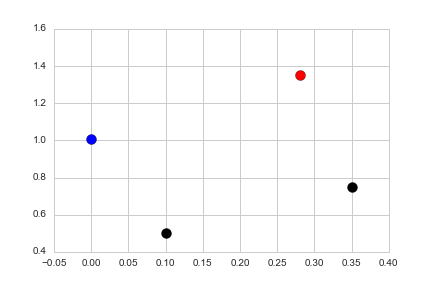
\includegraphics[scale=.3]{scatterplot.png} \end{center}


  Different pointwise distances $d(\boldx, \boldx') = \|\boldx - \boldx'\|_p$
  can be used.  Recall the definition of the
  $\ell_1$, $\ell_2$, and $\ell_{\infty}$ norm:
  \begin{eqnarray*}
     \| \mathbf{x} \|_1 = \sum_{j = 1}^m |x_i| \quad \quad\quad \| \mathbf{x} \|_2 = \sqrt{\sum_{j = 1}^m x_i^2 } \quad\quad\quad
     \| \mathbf{x} \|_{\infty} = \max_{j \in \{1, \ldots, m\}} |x_j|\\
  \end{eqnarray*}
  
  Also recall the definition of min-distance, max-distance,
  centroid-distance, and average-distance between two clusters (where $\bmu_{G}$
is the center of a cluster $G$):
%
\begin{eqnarray*}
    d_{\text{min}}(G, G') &=& \min_{\boldx  \in G, \boldx' \in G'} d(\boldx, \boldx')\\
    d_{\text{max}}(G, G') &=& \max_{\boldx  \in G, \boldx' \in G'} d(\boldx, \boldx')\\
    d_{\text{centroid}}(G, G') &=&  d(\bmu_{G}, \bmu_{G'})\\
    d_{\text{avg}}(G, G') &=&\frac{1}{|G| |G'|} \sum_{\boldx \in G}\sum_{\boldx'  \in G'} d(\boldx, \boldx')\\
  \end{eqnarray*}

  \begin{enumerate}
  \item Draw the 2D unit sphere for each norm,
  defined as $\mathcal{S} = \{\boldx \in \mathbb{R}^2: \|\boldx\| = 1 \}$. Feel free to do
  it by hand, take a picture and include it in your pdf.
\item  For each norm ($\ell_1, \ell_2, \ell_\infty$) and each clustering distance, specify which two clusters would
  be the first to merge.
\item Draw the complete dendrograms showing the order of agglomerations for the $\ell_2$ norm and each of the clustering distances. We have provided some code to make this easier for you. You are not required to use it.
  \end{enumerate}


\end{problem}

\newpage 
\subsection*{Solution: Hierarchical Clustering Clustering}

\begin{enumerate}
    \item Draw the 2D unit sphere for each norm,
        defined as $\mathcal{S} = \{\boldx \in \mathbb{R}^2: \|\boldx\| = 1 \}$. Feel free to do
        it by hand, take a picture and include it in your pdf.

        \begin{answer}
            \begin{figure}
                \centering
                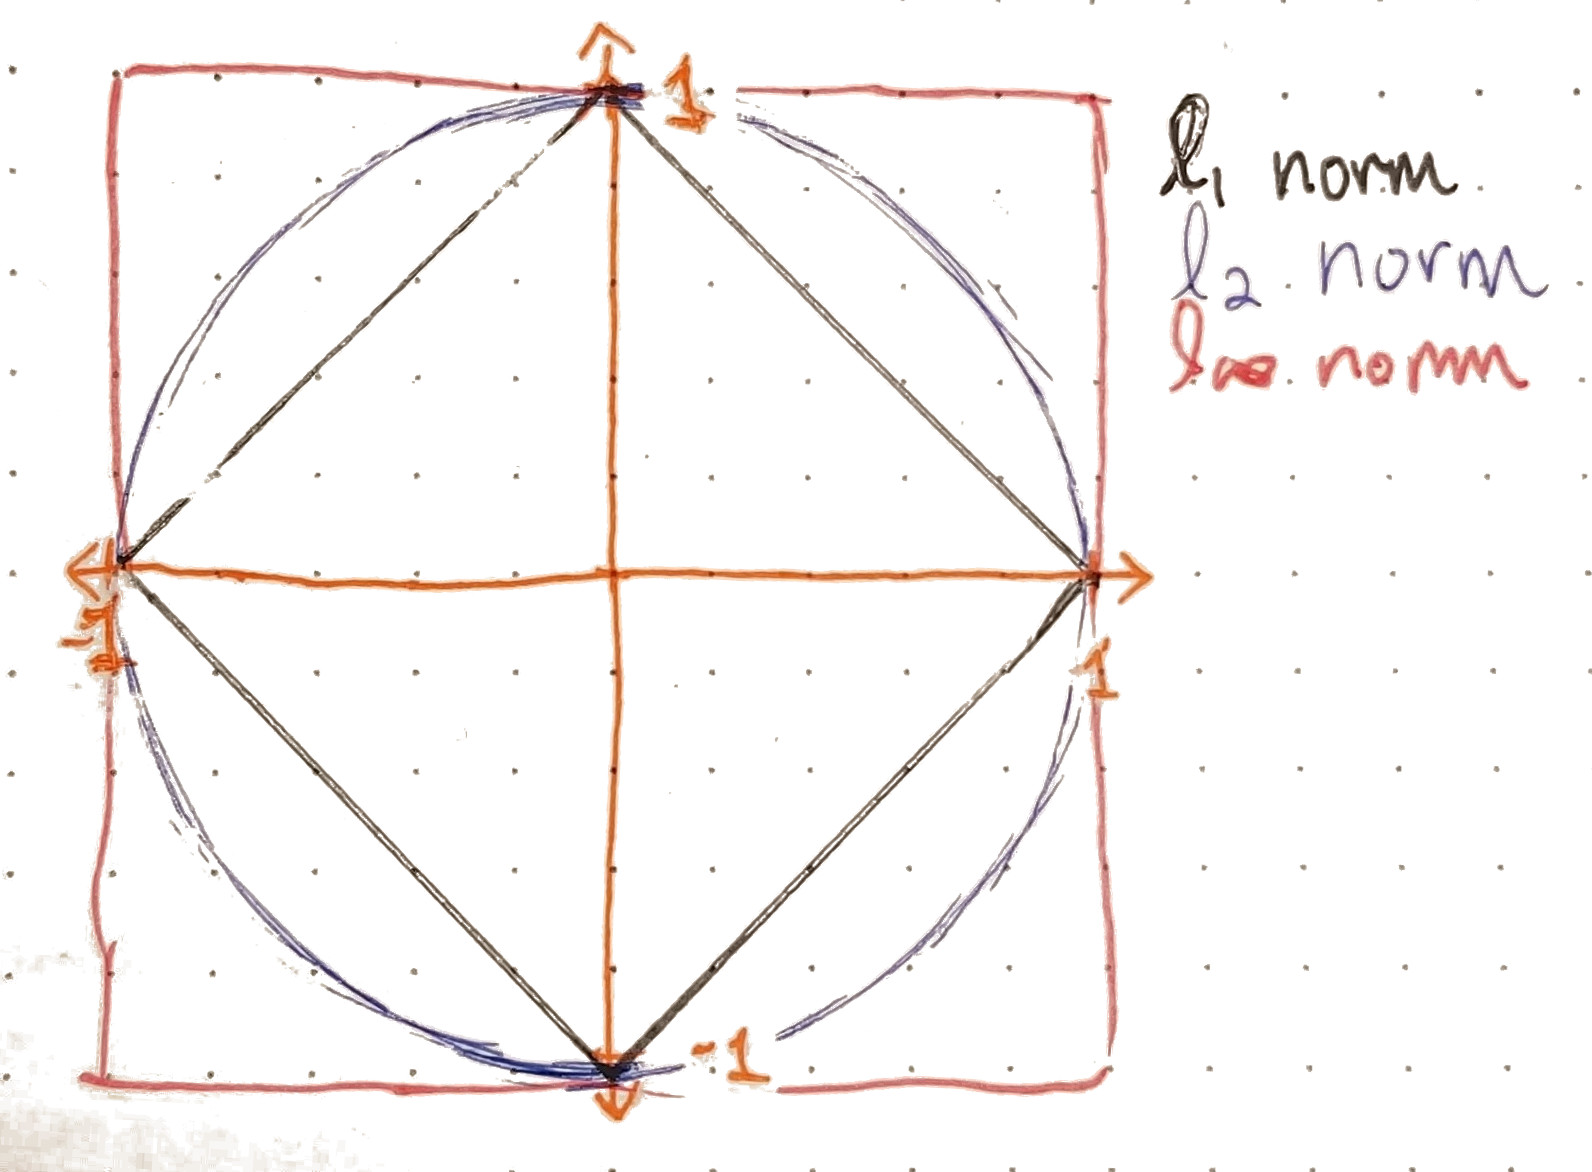
\includegraphics[width=0.25\textwidth]{p1_norms.jpg}
                \caption{Problem 1, 2d unit ball for l1, l2, and l$\infty$ norms}
                \label{p1}
            \end{figure}
        \label{P3 Means}

        See \cref{p1}
        \end{answer}

    \item  For each norm ($\ell_1, \ell_2, \ell_\infty$) and each clustering distance, specify which
        two clusters would be the first to merge.

        \begin{answer}
            See \cref{firstmerge}.

            \begin{table}[h]
                \centering
                \caption{First clusters to merge}
                \label{firstmerge}
                \begin{tabular}{@{}lllll@{}}
                    \toprule
                    & L1 norm     & L2 norm     & L$\infty$ norm     &  \\ \midrule
                    \multicolumn{1}{l|}{Min dist}      & black, blue & black, blue & red, blue   &
                    \\
                    \multicolumn{1}{l|}{Max dist}      & black, blue & red, blue & red, blue   &
                    \\
                    \multicolumn{1}{l|}{Avg dist}      & red, blue   & red, blue   & red, blue   &
                    \\
                    \multicolumn{1}{l|}{Centroid dist} & black, blue & black, blue & black, blue &
                    \\ \bottomrule
                \end{tabular}
            \end{table}
        \end{answer}

    \item Draw the complete dendrograms showing the order of agglomerations for the $\ell_2$ norm
        and each of the clustering distances. We have provided some code to make this easier for
        you. You are not required to use it.


        \begin{answer}
            \begin{figure}
                \centering
                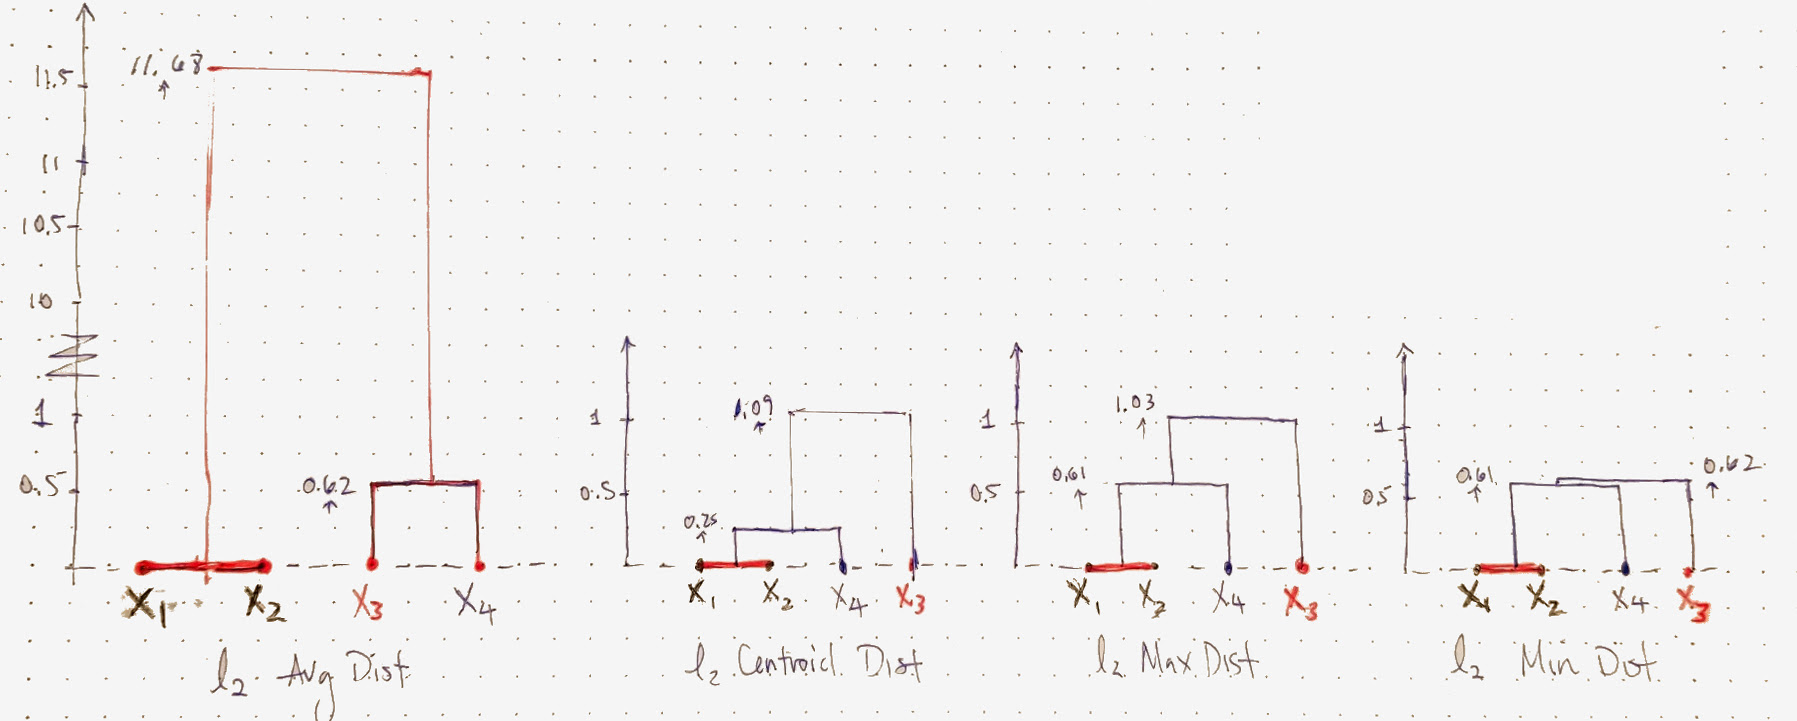
\includegraphics[width=\textwidth]{p1_dendograms.jpg}
                \caption{Problem 1, dendogram for clustering with l2 norm and each of the clustering
                distances.}
                \label{p1 dendo}
            \end{figure}

        See \cref{p1 dendo}


        For reference on distances used, see \cref{p1 dendo dist}

		\begin{table}
			\centering
			\begin{adjustbox}{max width=\textwidth}

				\begin{tabular}{@{}l|ll|ll|ll@{}}
					& \textbf{L1 norm} &              & \textbf{L2 norm} &              & \textbf{L∞ norm} &              \\ \midrule
					\textbf{min dist}      &                  & (merge dist) &                  & (merge dist) &                  & (merge dist) \\
					First merge            & black, blue      & 0.61         & black, blue      & 0.436        & red, blue        & 0.34         \\
					Second merge           & all              & 0.62         & all              & 0.440        & all              & 0.35         \\ \midrule
					\textbf{max dist}      &                  &              &                  &              &                  &              \\
					First merge            & black, blue      & 0.61         & red, blue        & 0.440        & red, blue        & 0.34         \\
					Second merge           & all              & 1.03         & all              & 0.869        & all              & 0.34         \\ \midrule
					\textbf{avg dist}      &                  &              &                  &              &                  &              \\
					First merge            & red, blue        & 0.62         & red, blue        & 0.440        & red, blue        & 0.34         \\
					Second merge           & all              & 11.68        & all              & 9.715        & all              & 9.24         \\ \midrule
					\textbf{centroid dist} &                  &              &                  &              &                  &              \\
					First merge            & black, blue      & 0.25         & black, blue      & 0.210        & black, blue      & 0.205        \\
					Second merge           & all              & 1.09         & all              & 0.657        & all              & 0.515       
				\end{tabular}
\end{adjustbox}
			\caption{Problem 1. Not asked for, but here are actual merge distances as output by python script for each combination of norms (distances) and clustering criteria}
			\label{p1 dendo dist}
		\end{table}
        \end{answer}

\end{enumerate}
\section*{Expectation-Maximization for Gaussian Mixture Models [7pts]}


In this problem we will explore expectation-maximization for the
Gaussian Mixture model.  Each observation $\boldx_i$ is a vector in
$\mathbb{R}^{D}$.  We posit that each observation comes from
\emph{one} mixture component.  For this problem, we will assume there
are $c$~components. Each component $k \in \{1, \ldots, c\}$ will be
associated with a mean vector $\mu_k \in R^{D}$ and a covariance
$\Sigma_k$.  Finally let the (unknown) overall mixing proportion of
the components be~$\btheta \in [0,1]^c$, where~${\sum_{k=1}^c
  \theta_k=1}$.

Our generative model is that each of the~$n$ observations comes from a
single component.  We encode observation $i$'s component-assignment as
a one-hot vector~${\boldz_i \in \{0,1\}^c}$ over components. This
one-hot vector is drawn from~$\btheta$; then, $\boldx_i$ is drawn
from~$N(\mu_{z_i}, \Sigma_{z_i})$. Formally documents are generated in two steps:
\begin{eqnarray*}
 \boldz_i &\sim& \text{Categorical}(\btheta) \\
 \boldx_i &\sim& N(\mu_{z_i}, \Sigma_{z_i})
\end{eqnarray*}


\begin{problem}
      ~

  \begin{enumerate}

  \item \textbf{Intractability of the Data Likelihood} Let $\phi_k$
    represent all the parameters associated with a component
    $(\mu_k,\Sigma_k)$.  We are generally interested in finding a set
    of parameters $\phi_k$ that maximize the data likelihood $\log
    p(\{x_i\}|\{phi_k\})$.  Expand the data likelihood to include the
    necessary sums over observations $x_i$ and latents $z_i$.  Why is
    optimizing this loss directly intractable?
    
\item \textbf{Complete-Data Log Likelihood} 

    Define the complete data for this problem to be $D =
    \{(\boldx_i, \boldz_i)\}_{i=1}^n$. Write out the complete-data (negative) log likelihood.
    \[\mcL(\btheta, \{\mu_k,\Sigma_k\}^c_{k=1}) =  -\ln p(D \given\btheta,
    \{\mu_k,\Sigma_k\}^c_{k=1}).\] 


\item \textbf{Expectation Step}
Our next step is to introduce a mathematical expression for $\boldq_i$, the posterior over the hidden topic variables~$\boldz_i$ conditioned on the observed data $\boldx_i$ with fixed parameters, i.e $p(\boldz_i | \boldx_i; \btheta, \{ \mu_k,\Sigma_k \}^c_{k=1})$.

\begin{itemize}
\item  Write down and simplify the expression for $\boldq_i$. 
\item  Give an algorithm for calculating $\boldq_i$ for all $i$, given the observed data~$\{\boldx_i\}^n_{i=1}$ and settings of the parameters~$\btheta$ and~$\{ \mu_k,\Sigma_k  \}^c_{k=1}$.

\end{itemize}

\item \textbf{Maximization Step}
Using the~$\boldq_i$ estimates from the Expectation Step, derive an update for maximizing the expected complete data log likelihood in terms of~$\btheta$ and~$\{ \mu_k,\Sigma_k \}^c_{k=1}$.

\begin{itemize}
    \item Derive an expression for the expected complete-data log likelihood in terms of $\boldq_i$.
    \item Find an expression for $\btheta$ that maximizes this expected complete-data log likelihood. You may find it helpful to use Lagrange multipliers in order to force the constraint $\sum \theta_k = 1$. Why does this optimized $\btheta$ make intuitive sense?
    \item Apply a similar argument to find the value of the $(\mu_k,\Sigma_k)$'s that maximizes the expected complete-data log likelihood. 
\end{itemize}

\item Finally, compare this EM approach to the generative model for
classification in Homework 2.  How are the computations similar?
Different? 

\end{enumerate}


  
\end{problem}

\subsection*{Solution EM for Gaussian Mixture Models}


\begin{enumerate}

    \item \textbf{Intractability of the Data Likelihood} 
        
        Let $\phi_k$ represent all the parameters associated with a component $(\mu_k,\Sigma_k)$.
        We are generally interested in finding a set of parameters $\phi_k$ that maximize the data
        likelihood $\log p(\{x_i\}|\{phi_k\})$.  Expand the data likelihood to include the necessary
		sums over observations $x_i$ and latents $z_i$.  Why is optimizing this
		loss directly intractable?

		\begin{answer}

    \begin{equation}
     \mathcal{N}(\bx \mid \bmu, \Sigma)
             = \frac{1}{\sqrt{(2\pi)^D|\bSigma|}}  \exp\left(-\frac 1 2 ({\mathbf x}-{\boldsymbol\mu})^\mathrm{T}{\boldsymbol\Sigma}^{-1}({\mathbf x}-{\boldsymbol\mu})\right)
    \end{equation}

        \begin{equation}
            \sum_{i=1}^n \sum_{k=1}^c \mu
            \left[ 
            \right] + const
        \end{equation}

        \begin{equation}
        \frac{\partial L_g}{\partial \bmu_k} = 
        \end{equation}
		\end{answer}

    \item \textbf{Complete-Data Log Likelihood} 

        Define the complete data for this problem to be $D = \{(\boldx_i, \boldz_i)\}_{i=1}^n$.
        Write out the complete-data (negative) log likelihood.  \[\mcL(\btheta,
        \{\mu_k,\Sigma_k\}^c_{k=1}) =  -\ln p(D \given\btheta, \{\mu_k,\Sigma_k\}^c_{k=1}).\] 

		\begin{answer}

		\end{answer}

    \item \textbf{Expectation Step}
        Our next step is to introduce a mathematical expression for $\boldq_i$, the posterior over
        the hidden topic variables~$\boldz_i$ conditioned on the observed data $\boldx_i$ with fixed
        parameters, i.e $p(\boldz_i | \boldx_i; \btheta, \{ \mu_k,\Sigma_k \}^c_{k=1})$.

        \begin{itemize}
            \item  Write down and simplify the expression for $\boldq_i$. 

				\begin{answer}

				\end{answer}

            \item  Give an algorithm for calculating $\boldq_i$ for all $i$, given the observed
                data~$\{\boldx_i\}^n_{i=1}$ and settings of the parameters~$\btheta$ and~$\{
                \mu_k,\Sigma_k  \}^c_{k=1}$.

				\begin{answer}

				\end{answer}

		\end{itemize}

	\item \textbf{Maximization Step}
		Using the~$\boldq_i$ estimates from the Expectation Step, derive an update for maximizing
		the expected complete data log likelihood in terms of~$\btheta$ and~$\{ \mu_k,\Sigma_k
		\}^c_{k=1}$.

		\begin{itemize} 
			\item Derive an expression for the expected complete-data log likelihood in
				terms of $\boldq_i$.

				\begin{answer}

				\end{answer}

			\item Find an expression for $\btheta$ that maximizes this expected complete-data log
				likelihood. You may find it helpful to use Lagrange multipliers in order to force
				the constraint $\sum \theta_k = 1$. Why does this optimized $\btheta$ make intuitive
				sense?

				\begin{answer}

				\end{answer}
			\item Apply a similar argument to find the value of the $(\mu_k,\Sigma_k)$'s that
				maximizes the expected complete-data log likelihood.  
				\begin{answer}

				\end{answer}

		\end{itemize}

	\item Finally, compare this EM approach to the generative model for classification in Homework
		2.  How are the computations similar?  Different? 

		\begin{answer}

		\end{answer}

\end{enumerate}


\newpage

\section*{K-Means [15 pts]} % FDV: Any more interesting data sets?  

For this problem you will implement  K-Means clustering from scratch. Using \texttt{numpy} is fine,
but don't use a third-party machine learning implementation like \texttt{scikit-learn}. You will
then apply this approach to clustering of image data.  



We have provided you with the MNIST dataset, a collection of handwritten digits used as a benchmark
of image recogntion (you  can learn more about the data set at
\url{http://yann.lecun.com/exdb/mnist/}). The MNIST task is widely used in supervised learning, and
modern algorithms with neural networks do very well on this task. 

Here we will use MNIST unsupervised learning. You have been given representations of 6000 MNIST
images, each of which are $28\times28$ greyscale handwritten digits. Your job is to implement
K-means clustering on MNIST, and to test whether this relatively simple algorithm can cluster
similar-looking images together.

~
\begin{problem}
The given code loads the images into your environment as a 6000x28x28 array.

\begin{itemize}
    \item Implement K-means clustering
        from different random initializations and for several values of $K$ using the $\ell_2$ norm
        as your distance metric. (You should feel free to explore other metrics than the $\ell_2$
        norm, but this is strictly optional.)  Compare the K-means objective for different values of
        K and across random initializations.
%
\item For three different values of K,
    and a couple of random restarts for each, show the mean images for each cluster (i.e., for the
    cluster prototypes), as well as the images for a few representative images for each cluster. You
    should explain how you selected these representative images. To render an image, use the pyplot
    \texttt{imshow} function. 

\item Are the results wildly different for different restarts and/or different values of K?  For one
    of your runs, plot the K-means objective function as a function of iteration and verify that it
    never increases.

\end{itemize}


As in past problem sets, please include your plots in this
document. (There may be several plots for this problem, so feel free
to take up multiple pages.)




\end{problem}
\subsection*{Solution: K-Means}

\begin{itemize}
\item Implement K-means clustering
from different random initializations 
and for several values of $K$ using the 
$\ell_2$ norm as your
distance metric. (You should feel free to explore other metrics 
than the $\ell_2$ norm, but this is strictly optional.)  Compare the 
K-means objective for different values of K and across random
initializations.
%
\begin{answer}

    From the following table \ref{my-label} we may observe that the objective decreases as K increases.
    Additionally, for each run of K, the final objective (cost) is fairly consistent, without large
    variations, compared to the changes in final cost between different K values.

    \begin{table}[H]
        \centering
        \caption{K-Means l2 objective for different values of K. Normalized = divided by 6000*28*28,
        for readability.}
        \label{my-label}
        \begin{tabular}{@{}lll@{}}
            \toprule
            K (\# clusters) & Objective (normalized) & Objective  \\ \midrule
            2               & 2.2632                 & 10646092.8 \\
            2               & 2.2631                 & 10645622.4 \\
            2               & 2.2631                 & 10645622.4 \\
            5               & 2.1117                 & 9933436.8  \\
            5               & 2.1191                 & 9968246.4  \\
            5               & 2.1183                 & 9964483.2  \\
            10              & 1.99                   & 9360960    \\
            10              & 1.9888                 & 9355315.2  \\
            10              & 1.9868                 & 9345907.2  \\
            15              & 1.9222                 & 9042028.8  \\
            15              & 1.9212                 & 9037324.8  \\
            15              & 1.9187                 & 9025564.8  \\ \bottomrule
        \end{tabular}
    \end{table}

\end{answer}

\item For three different values of K, and a couple of random restarts for each, show the mean
    images for each cluster (i.e., for the cluster prototypes), as well as the images for a few
    representative images for each cluster. You should explain how you selected these representative
    images. To render an image, use the pyplot \texttt{imshow} function. 

\begin{answer}

In the representative images, each row indicates images from one cluster.
For each row, the three left images are chosen as the three closest (as defined
by the objective function) to the centroid, and the three right images are the three worst scoring images.

~~~~~~~~~~~~~~~~~ TODO REMEMBER to comment out images below for final submission!!
%\begin{figure}[h]
        %\centering
        %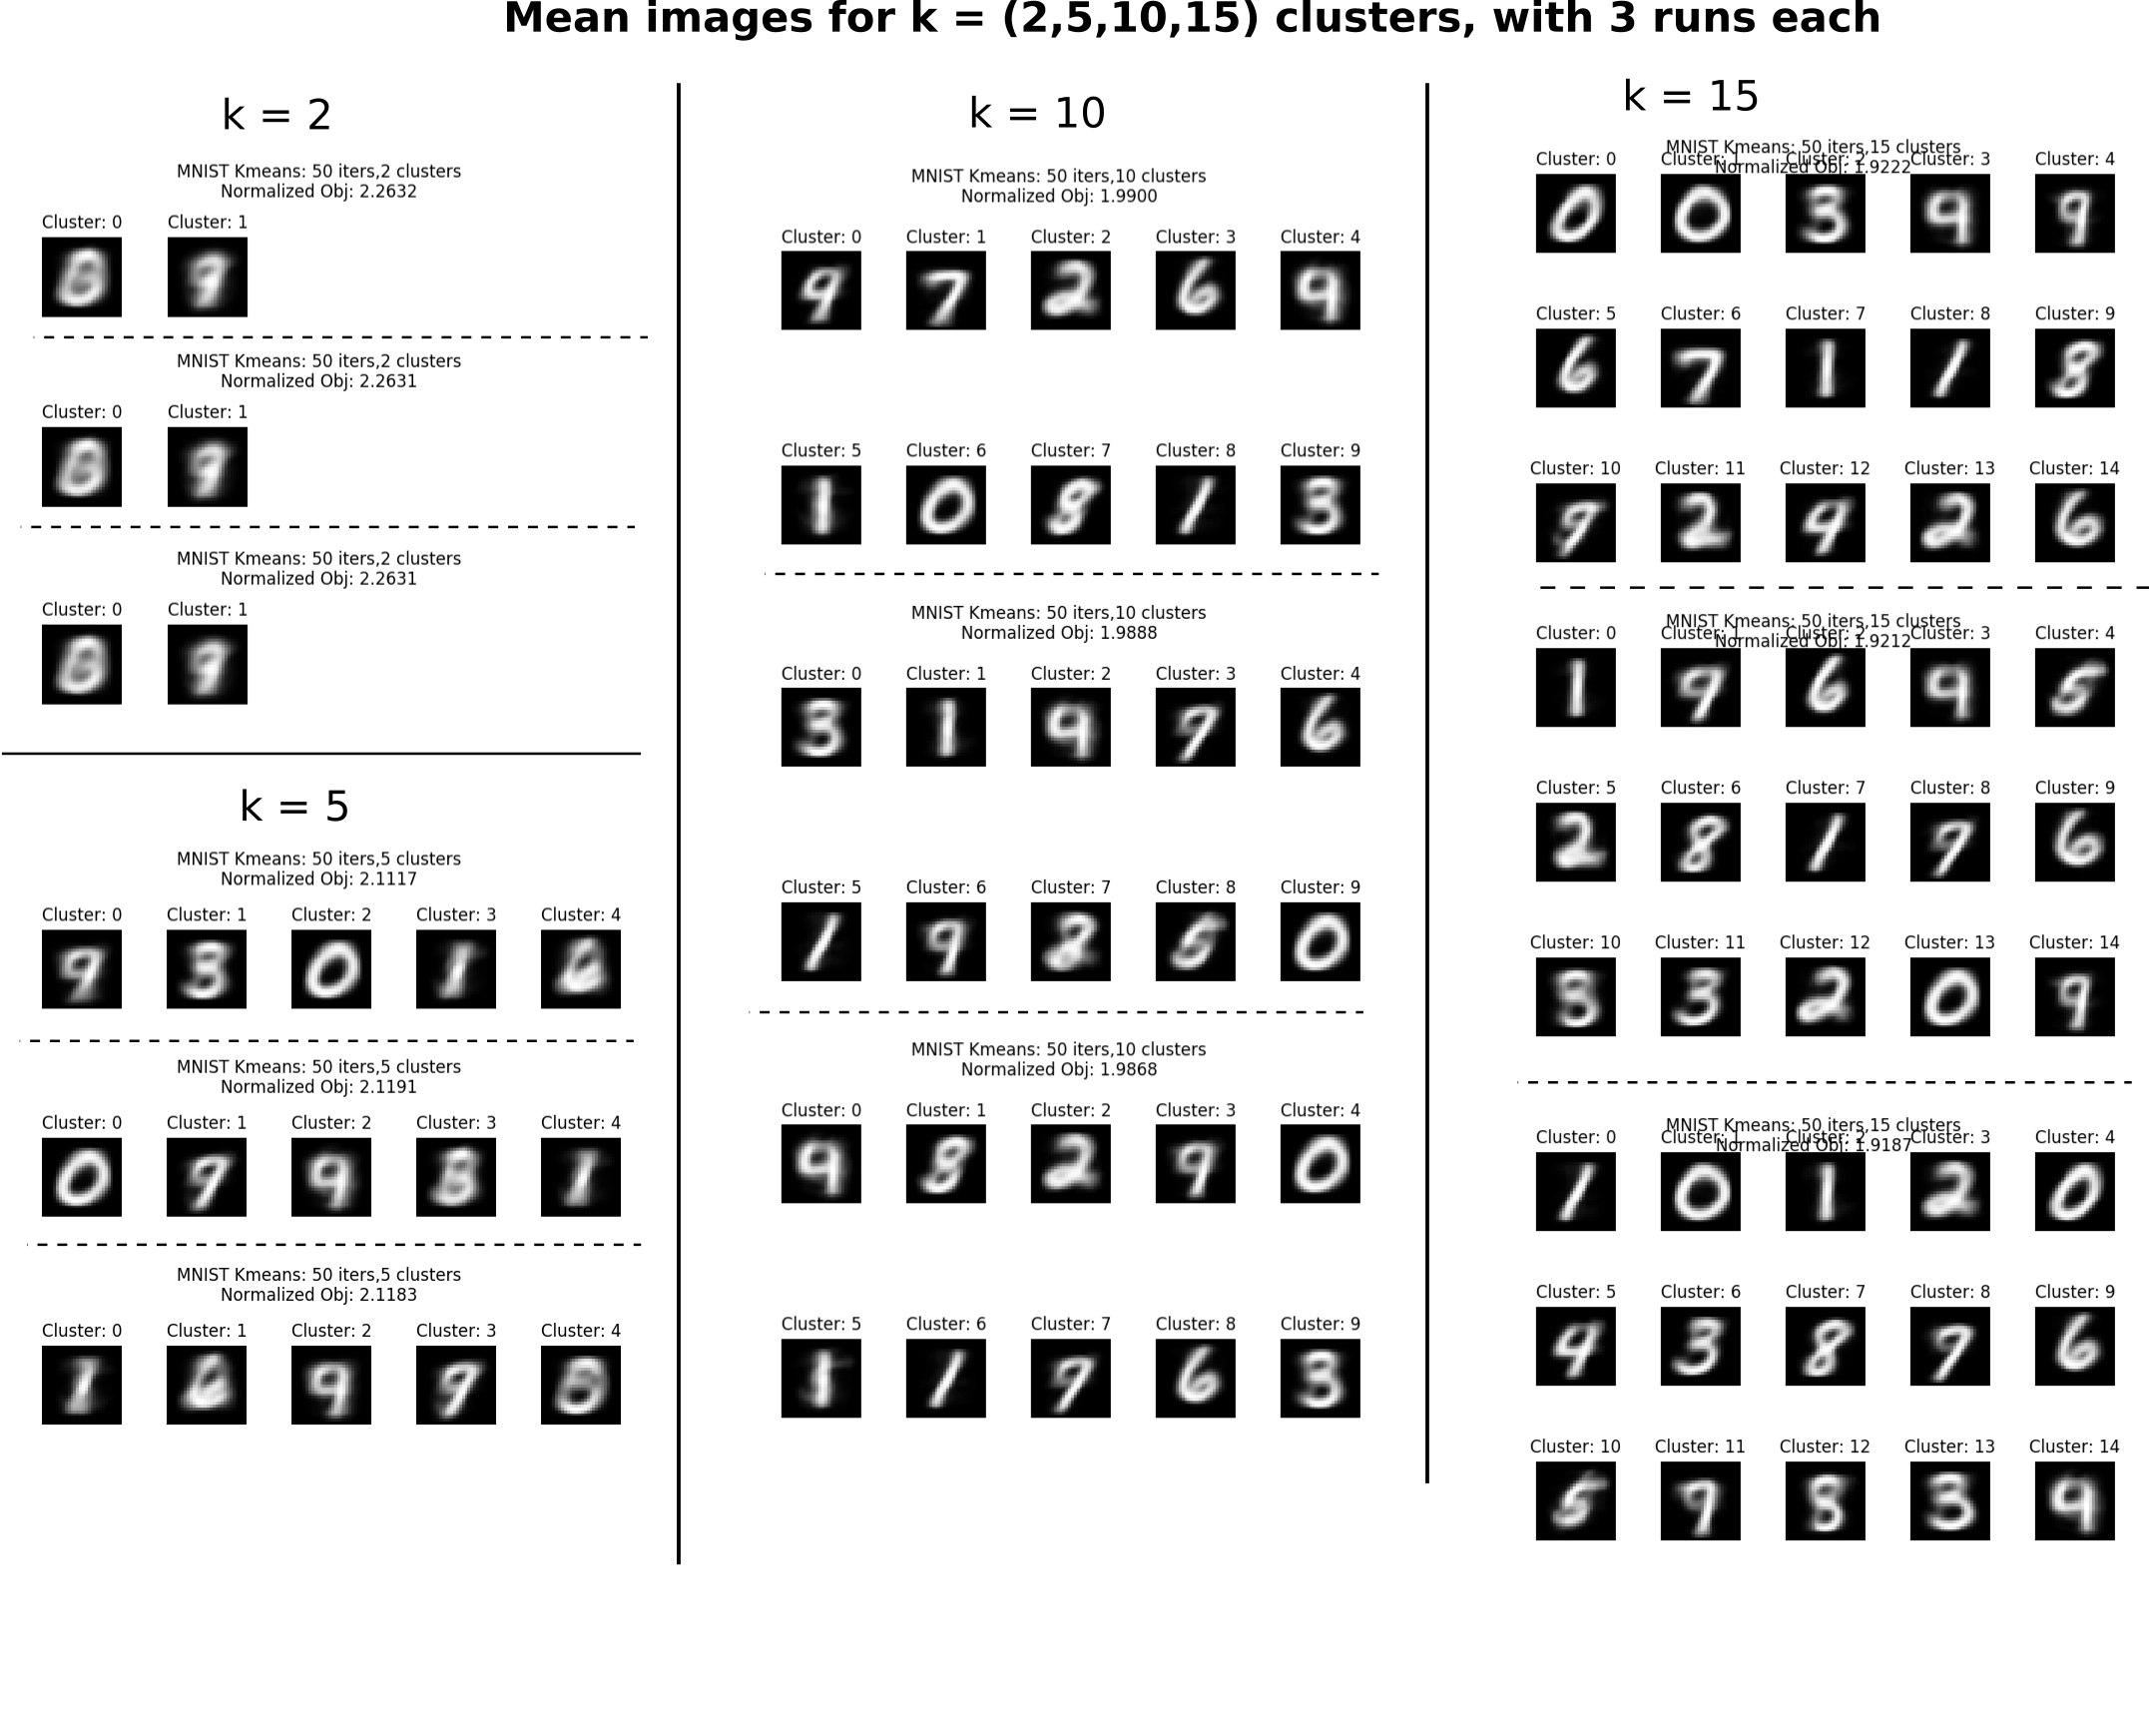
\includegraphics[width=\textwidth,height=0.28\paperheight]{p3_means.png}
        %\caption{Problem 3, Mean images, with a bonus K=15 centroid runs.}
        %\label{P3 Means}

        %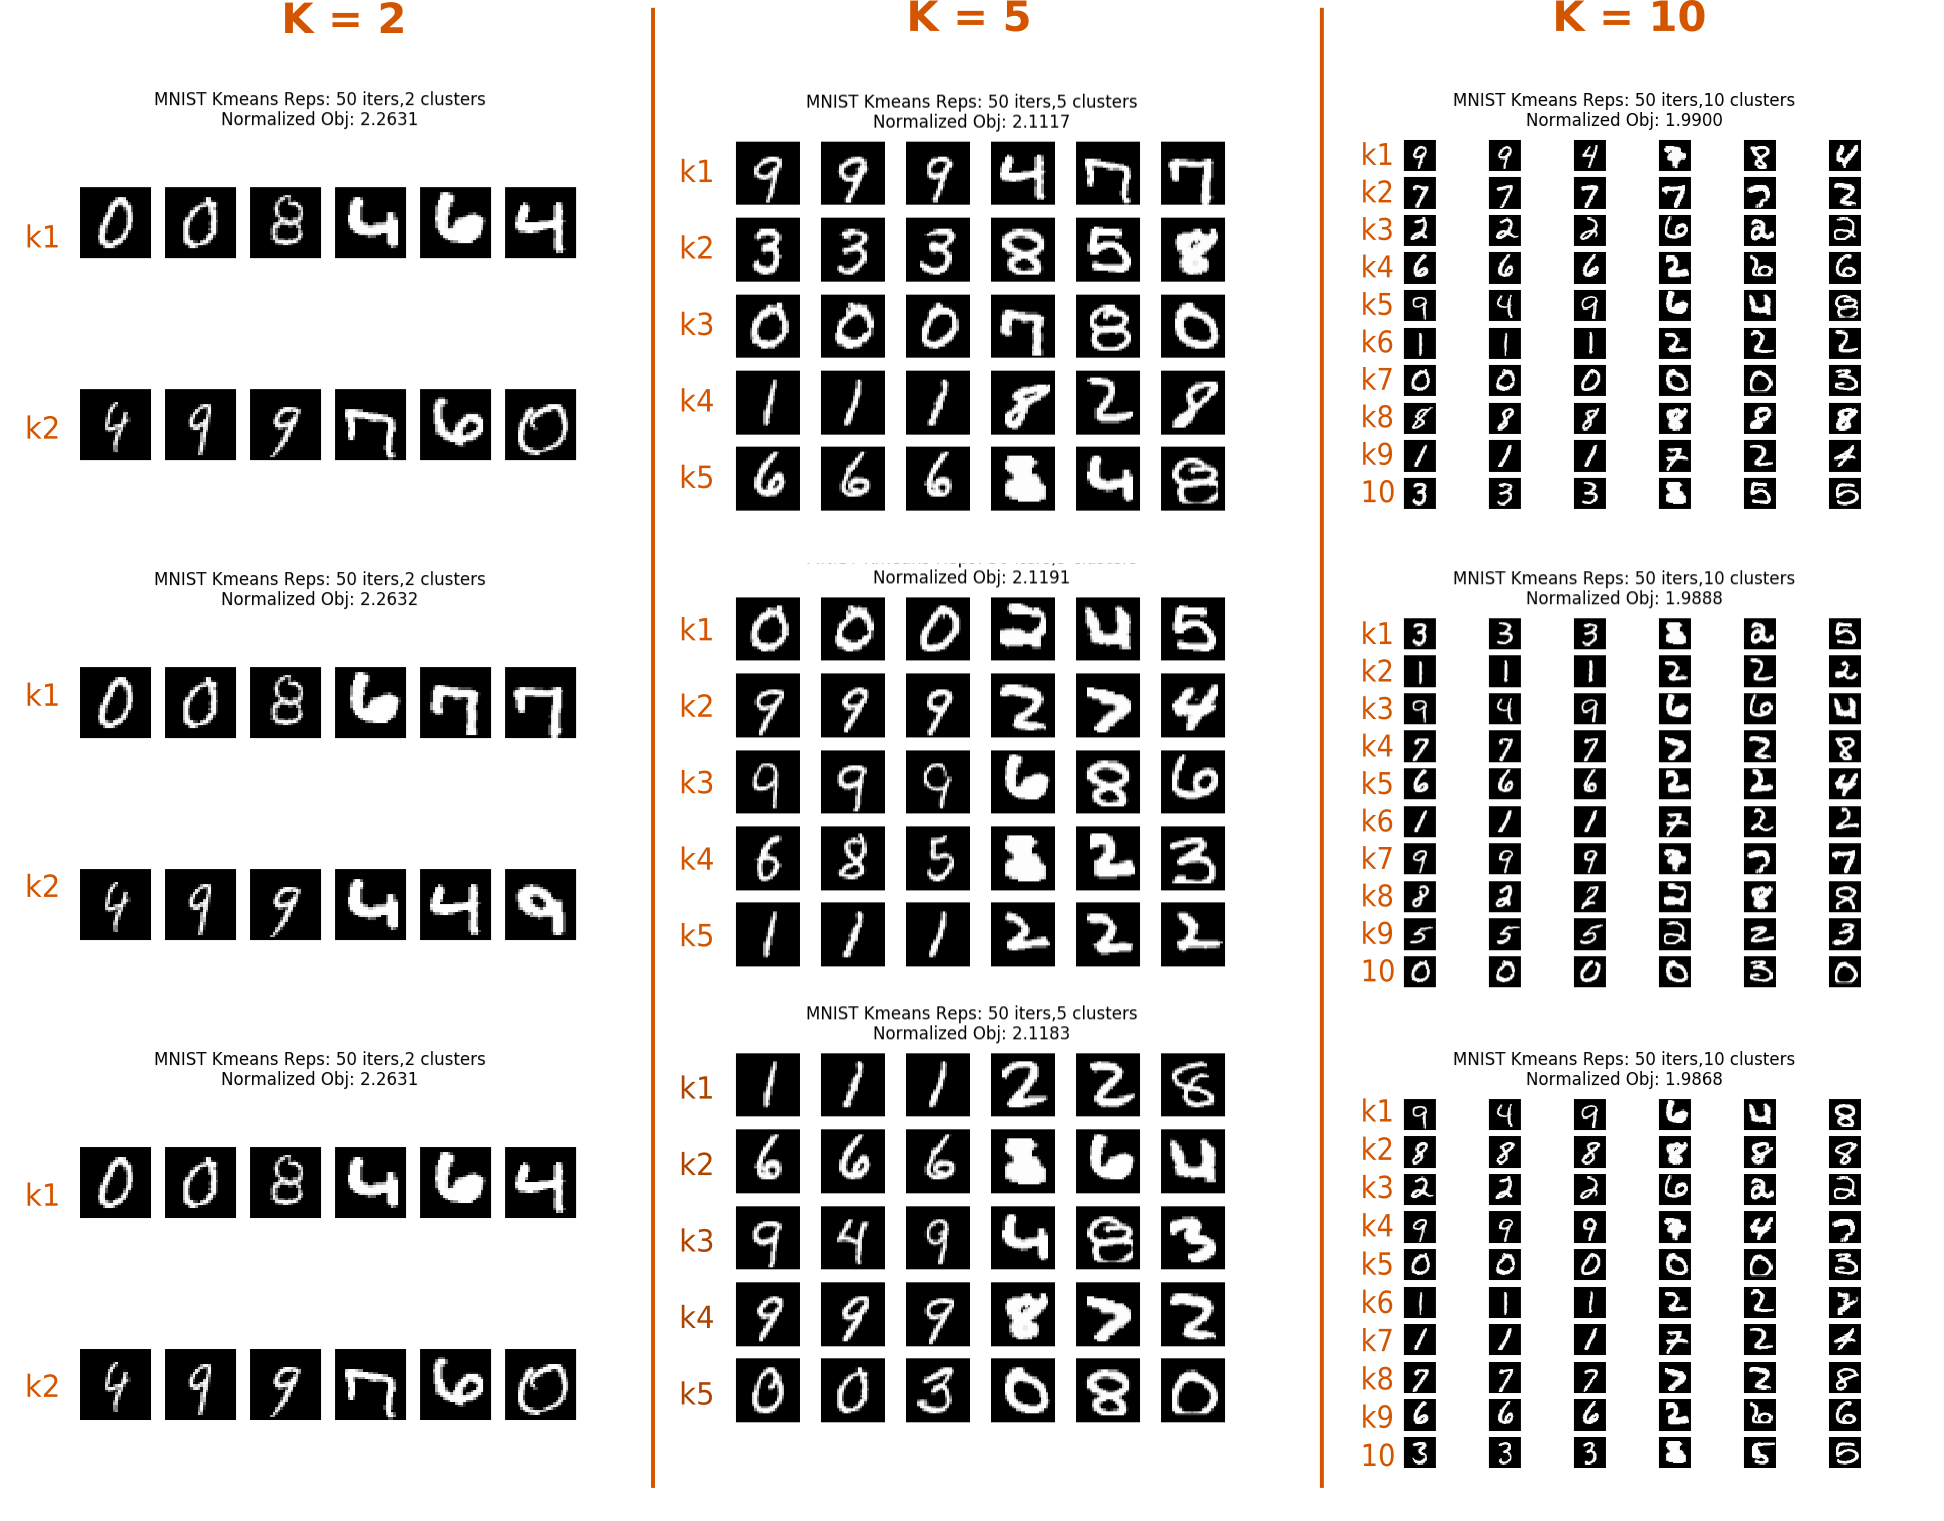
\includegraphics[width=\textwidth,height=0.5\paperheight]{p3_reps.png}
        %\caption{Problem 3, Representative images, note that K=15 is not depicted here. Left 3 are
        %closest to centroid by l2 norm, right 3 are furthest.}
        %\label{P3 Reps}
%\end{figure}

\end{answer}


\item Are the results wildly different for different
restarts and/or different 
values of K?
For one of your runs, plot the K-means objective function as a function of iteration and verify that
it never increases.

\begin{answer}
        Compared to the k-means objective (as answered in part 1), The representative images /
        cluster results do seem to vary noticeably between runs, aside from the K=2 case, which
        exhibits little variation.  The results do vary even more for different values of K; for
        K=10, the mean images will sometimes miss entire numbers, while for k=15 we will get repeats
        of a few of the values
        even if we get most of the digits. 

        For the following, we graph a run of the KMeans algorithm for K=10 clusters. The run
        converged after 24 iterations (where by converge I set it to mean that the previous and
        current objective value did not change). Although a bit hard to see, 
    \begin{figure}[ht]
        \centering
        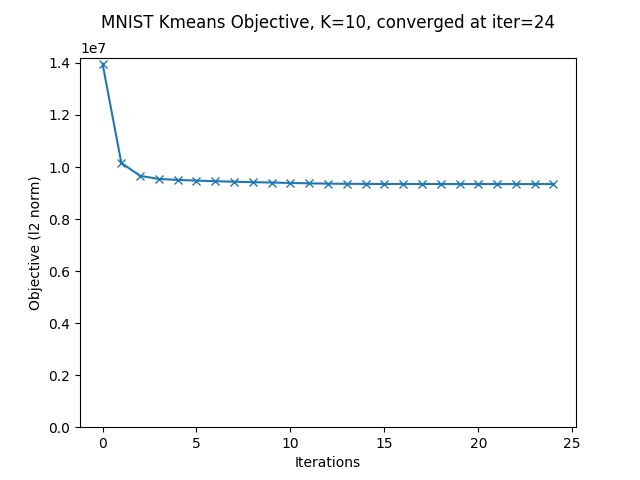
\includegraphics[width=0.5\textwidth]{p3_costvsiter.png}
        \caption{Problem 3: Verification that K-means objective function decreases as a function of
        iteration}
        \label{cost}
    \end{figure}
\end{answer}

\end{itemize}

%Figure out how to load it into your environment and turn it into a set of
%vectors.  Run K-Means on it for a few different~$K$ and show some results from
%the fit.  What do the mean images look like?  What are some representative
%images from each of the clusters?  Are the results wildly different for
%different restarts and/or different~$K$?  Plot the K-Means objective function
%(distortion measure) as a function of iteration and verify that it never
%increases.

%\subsection*{4. Implement K-Means++ [4 pts]} mplement K-Means++ and see if it
%gives you more satisfying initializations for K-Means.  Explain your findings.

\newpage
\begin{problem}[Calibration, 1pt]
Approximately how long did this homework take you to complete?
\end{problem}

~20-30 hours
\subsection*{Name, Email, and Collaborators}

Name: Nao Ouyang

Email: nouyang@g.harvard.edu    

Collaborators:
Eric
Buse
Philip
David


\end{document}

% vim --servername vim test.tex
